\chapter{Parser}

In this chapter the requirements of NISSE will be presented, along with the context free grammar(CFG) of NISSE.
\section{Requirements}
Requirements of the NISSE parser:
\begin{itemize}
	\item The parser should be able to receive tokens from the lexer, which it can then convert into a parse tree.
	\item It should be able to report useful error messages, if the user has written something illegal according to the CFG of NISSE.
	\item The CFG should be LL(1) in order to speed up the compiler.
	\item The CFG should also not be ambiguous, so that we can make a parser for it. Because the CFG is LL(1) (as per the previous requirement) the CFG is also not ambiguous as per the definition of LL(1).
\end{itemize}
\newpage
\section{CFG}
\begin{lstlisting}[frame=single, caption={CFG of NISSE in EBNF.}, label={lst:ebnf}, language=NISSE]
SS            = {Blocks} ;
Blocks        = BeginBlock {Lines} EndBlock 
              | SettingBlock ;
Lines         = SettingBlock 
              | Numeration
              | Itemlist 
              | Plains eol ;
Numeration    = nlist (Plains eol | Numeration) ;
Itemlist      = blist (Plains eol  | Itemlist) ;
BeginBlock    = beginkwd BEBlock eol ;
EndBlock      = endkwd BEBlock eol+ ;
BEBlock       = lcurly [space] char [space] [pipe char [space]] rcurly ;
SettingBlock  = settingkwd lcurly ShortIdent [space] pipe [space] char [space] rcurly eol;
Plains        = (ShortBlock | CharAll)+ ;
ShortBlock    = format_kwd lcurly [space] [ShortIdents] Plains rcurly ;
ShortIdents   = {ShortIdent}+ pipe ;
ShortIdent    = Kwd [space] colon [space] (char | digit) [space] ;
Kwd           = atsign char ;
CharAll       = colon 
              | digit 
              | scolon 
              | percent 
              | fslash 
              | bslash 
              | char 
              | space ;
\end{lstlisting}

Listing \ref{lst:ebnf} shows the CFG for NISSE in Extended Backus Naur Form, henceforth EBNF. It should be read as follow:
\begin{center}
\begin{tabular}{|l|l|}
\hline 
Usage & Notation \\ 
\hline 
definition & = \\ 
\hline 
concatenation & ,	 \\ 
\hline 
termination & ; \\ 
\hline 
alternation & | \\ 
\hline 
option & [ ... ] \\ 
\hline 
repetition & { ... } \\ 
\hline 
grouping & ( ... ) \\ 
\hline 
terminal string & " ... " \\ 
\hline 
terminal string & ' ... ' \\ 
\hline 
comment & (* ... *) \\ 
\hline 
special sequence & ? ... ? \\ 
\hline 
exception & - \\ 
\hline 
\end{tabular}
\end{center}
An example is the line \lstinline!S = a {b}+ [ {c}+ ] ( a | b ) ;! that translates to \lstinline!S = a! followed by at least one \lstinline!b! followed by none or at least one \lstinline!c! followed by \lstinline!a! or \lstinline!b!. The special sequence is used for writing anything that is not directly EBNF. An example is \lstinline!char = ? a-zA-Z ? ;! where all letters from a to z is defined both capitol and non-capitol.

NISSE's grammar is able to construct everything that is required of NISSE. \\
Let's look at one of the previous examples:

\begin{lstlisting}[frame=single]
Input:
@begin{fade|slide}
    Hello World
@end{slide}
\end{lstlisting}

The parse tree for this would look like: 

\begin{figure}[! h]
\centering
	 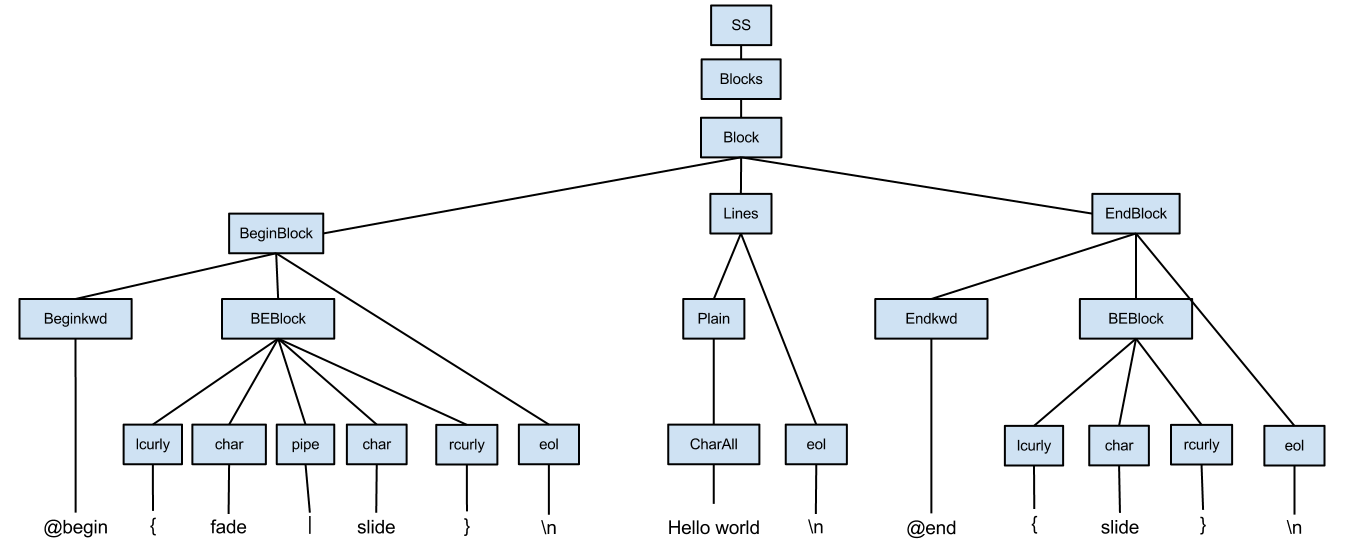
\includegraphics[width=300px]{images/ebnfexample.png}
		 \caption{Parse tree for a simple slide.}	
	\label{fig:Parsetree}
\end{figure}
The figure \ref{fig:Parsetree} shows how it would parse the tree, with the input in a slide of �Hello World''. 